\section{Recovering hidden marginals}
\label{sec:hiddenMarginals}

\begin{figure}
  \centering
  \subfigure[Bottleneck] {
    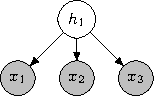
\includegraphics[width=0.35\columnwidth]{figures/three-view.pdf}
    \label{fig:bottleneck}
  }
  \hspace{2em}
  \subfigure[Exclusive views]{
    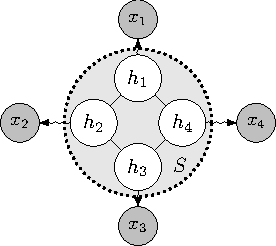
\includegraphics[width=0.35\columnwidth]{figures/exclusive-views.pdf}
    \label{fig:exclusive-views}
  }

  \caption{
    \label{fig:bottleneckExclusiveViews}
  (a) A bottleneck $h_1$ has three conditionally independent views $x_1,x_2,x_3$.
  %using tensor factorization \citep{anandkumar13tensor}.
  (b) A bidependent subset $S$ has exclusive views $\{x_1,x_2,x_3,x_4\}$.
  }
\end{figure}

%In this section, we will develop a consistent parameter estimate for a class of directed graphical models.
%The conditional moments $\mOpp{v}{i} \eqdef \Pr(x_v \mid h_i)$
%recovered from {\TensorFactorize}, are not the underlying parameters.
  %Once we recover the conditional moments $\mOpp{v}{j} \eqdef \Pr(x_v
  %\given h_j)$ for some $v, j$, we present a systematic approach to learn the
  %conditional probability tables for every clique for a class of directed
  %graphical models.
Having recovered conditional moments $\mOpp{v}{i} \eqdef \Pr(x_v \mid h_i)$,
we now seek to compute the marginal distribution of sets of hidden variables
$Z_S \eqdef \Pr(\bh_S)$.
%taking us one step closer to the actual model parameters.

%%%%%%%%%%%%%%%%%%%%%%%%%%%%%%%%%%%%%%%%%%%%%%%%%%%%%%%%%%%%
%\subsection{Example: directed grid model}
%\label{sec:directedExample}

\paragraph{Example}

%The model has eight observed variables $x^a_1, x^b_1 \cdots, x^a_4, x^b_4$ and four
  %hidden variables $h_1, \ldots, h_4$.
%The parameters of this model are the conditional probability tables
%$\pi \eqdef \Pr(h_1) \in \Re^k, T \eqdef \Pr(h_2 | h_1) = \Pr(h_3 | h_1) \in \Re^{k \times k},
%V \eqdef \Pr(h_4 | h_2, h_3) \in \Re^{k \times k \times k}$ and $O \eqdef \Pr(x^a_i | h_i)
%=  \Pr(x^b_i | h_i) \in \Re^{d \times k}$. 

%\paragraph{Estimating $O$}
%Since the observed variables $x^a_1, x^b_1, x^a_2$ are
%  conditionally independent given $h_1$, we can $\TensorFactorize$ from
%  \sectionref{setup} to recover $O$.

%\paragraph{Estimating $\pi$}
%The moments of $x^a_1$, $\mO_1 \eqdef \Pr(x^a_1)$ are directly related to
%  $\pi$ by a linear system: $\mO_1 = O \pi$. 
%If $O$ has full column rank, we can recover $\pi$ by taking the pseudoinverse: $\pi = O\pinv  \mO_1$.

%\paragraph{Estimating $T$}

To gain some intuition, consider the directed grid model from \figureref{approach}.
We can express the observed marginals $\mO_{12} \eqdef \Pr(x^a_1, x^a_2) \in \Re^{d \times d}$
as a linear function of the hidden marginals $\mH_{12} \eqdef \Pr(h_1, h_2) \in \Re^{k \times k}$,
where the linear coefficients are based on the conditional moments
$\mOpp{1}{1},\mOpp{2}{2} \in \Re^{d \times k}$:
%down the moments of $x^a_1, x^a_2$,
\begin{align*}
\mO_{12} = \mOpp{1}{1} \mH_{12} \mOppt{2}{2}.
\end{align*}
We can then solve for $\mH_{12}$ by matrix inversion:
\begin{align*}
\mH_{12} = \mOppi{1}{1} \mO_{12} \mOppit{2}{2}.
\end{align*}
%$T$ can be recovered from the $\mH_{12}$ by renormalizing the columns.

%\paragraph{Estimating $V$}
%Finally, we can estimate $V$ by renormalizing the hidden marginals
%$\mH_{234} \eqdef \Pr(h_2, h_3, h_4)$ from the third-order moments
%$\mO_{234} \eqdef \Pr(x^a_2, x^a_3, x^a_4)$:
%\begin{align*}
%  \mO_{234} = \mH_{234}(O, O, O) \quad\Rightarrow\quad
%  \mH_{234} = \mO_{234}(O\pinv , O\pinv , O\pinv ).
%\end{align*}

%%%%%%%%%%%%%%%%%%%%%%%%%%%%%%%%%%%%%%%%%%%%%%%%%%%%%%%%%%%%
\subsection{Exclusive views}
\label{sec:general}

%The intuitions of the directed grid generalize readily to general graphs.
%The key property required for our algorithm to work is as follows:
For which subsets of hidden nodes can we recover the marginals?  The following
definition offers a characterization:
\begin{definition}[Exclusive views]
  \label{def:exclusive-views}
Let $S \subseteq \bh$ be a subset of hidden variables.
We say $h_i \in S$ has an exclusive view $x_v$
  if the two conditions hold:
  (i) there exists some observed variable
  $x_{v}$ which is conditionally independent of the others $S \backslash \{ h_i \}$ given $h_i$ (\figureref{exclusive-views}),
  and (ii) the conditional moment matrix $\mOpp{v}{i} \eqdef
  \Pr(x_{v} \mid h_i)$ has full column rank $k$ and can be recovered.
We say that $S$ has the \emph{exclusive views property} if every $h_i \in S$ has an exclusive view.
%If every hidden clique has the exclusive views property, then we say that $\sG$ does as well.
\end{definition}

%%%%%%%%%%%%%%%%%%%%%%%%%%%%%%
\paragraph{Estimating hidden marginals}

We now show that if a subset of hidden variables $S$ has the exclusive views property,
then we can recover the marginal distribution $\Pr(\bh_S)$.
Consider any $S = \{h_{i_1}, \ldots, h_{i_m}\}$ with the exclusive views property. Let
  $x_{v_j}$ be an exclusive view for $h_{i_j}$ in $S$ and define $\sV
  = \{x_{v_1}, \ldots, x_{v_m}\}$. % be a set of exclusive views for the clique $S$.
By the exclusive views property,
the marginal over the observed variables $\Pr(\bx_\sV)$
factorizes according to the marginal over the hidden variables $\Pr(\bh_S)$
times the conditional moments:
\begin{align*}
  \mO_\sV 
  &\eqdef \Pr(\Sx{\sV}) \\
  &= \sum_{\vh_S} \Pr(\Sh{S}) 
                    \Pr(x_{v_1} \given h_{i_1}) \cdots \Pr(x_{v_m} \given h_{i_m}) \\
  &= Z_{S}(\mOpp{v_1}{i_1},\dots,\mOpp{v_m}{i_m}) \\
  &= Z_{S}(\mOppAll),
\end{align*}
where $\mOppAll = \mOpp{v_1}{i_1} \otimes \cdots \otimes \mOpp{v_m}{i_m}$ is the tensor product of
all the conditional moments.
Vectorizing, we have that
$Z_S \in \Re^{k^m}$,
$M_\sV \in \Re^{d^m}$,
and $\mOppAll \in \Re^{d^m \times k^m}$.
Since each $\mOpp{v}{i}$ has full column rank $k$,
the tensor product $\mOppAll$ has full column rank $k^m$.
Succinctly, $\mO_\sV$ (which can be estimated directly from data)
is a linear function of $Z_S$ (what we seek to recover).
We can solve for the hidden marginals $Z_S$ simply by multiplying $\mO_\sV$ by the pseudoinverse of
$\mOppAll$:
\begin{align*}
  Z_{S} &= \mO_\sV(\mOpp{v_1}{i_1}\pinv,\cdots,\mOpp{v_m}{i_m}\pinv).
\end{align*}

\algorithmref{learnMarginals} summarizes the procedure, \LearnMarginals.
Given $Z_S$, the conditional probability tables for $S$ can easily be
obtained via renormalization.
\begin{theorem}[Hidden marginals from exclusive views]
If $S \subseteq \bx$ is a subset of hidden variables with the exclusive views property,
then \algorithmref{learnMarginals} recovers the marginals $Z_S
= \Pr(\bh_S)$ up to a global relabeling of the hidden variables
determined by the labeling from $\TensorFactorize$.
\end{theorem}

\begin{algorithm}
  \caption{\LearnMarginals~(pseudoinverse)}
  \label{algo:learnMarginals}
  \begin{algorithmic}
    \REQUIRE Hidden subset $S = \{ h_{i_1}, \dots, h_{i_m} \}$ with exclusive views $\sV = \{ x_{v_1}, \dots, x_{v_m} \}$
    and conditional moments $\mOpp{v_j}{i_j} = \Pr(x_{v_j} \mid h_{i_j})$.
    \ENSURE Marginals $Z_S = \Pr(\bh_S)$.
      %\STATE Identify exclusive views $\Sx{\sV} = \{x_{v_1}, \dots, x_{v_m}\}$.
      \STATE Return $\mH_S \gets \mO_{\sV}( \mOpp{v_1}{i_1}\pinv, \dots, {\mOpp{v_m}{i_m}}\pinv )$.
  \end{algorithmic}
\end{algorithm}

%%%%%%%%%%%%%%%%%%%%%%%%%%%%%%
\paragraph{Relationship to bottlenecks}

%We have shown how to estimate the parameters of any clique that possesses the exclusive
  %views property (\definitionref{exclusive-views}).
  %But in a general graph, which cliques have this property?
  %To provide intuition, we will provide more interpretable sufficient conditions
  %and examples.

The bottleneck property allows recovery of conditional moments,
and the exclusive views property allows recovery of hidden marginals.
But we will now show that the latter property is in fact implied by the former
property for special sets of hidden variables, which we call bidependent
sets (in analogy with biconnected components),
in which conditioning on one variable does not break the set apart:
\begin{definition}[Bidependent set]
We say that a subset of nodes $S$ is \emph{bidependent} if
conditioned on any $a \in S$, there is an active trail between any other two nodes $b,c \in S$.
\end{definition}
Note that all cliques are bidependent, but bidependent sets can have more conditional independences
(e.g., $\{h_1,h_2,h_3\}$ in \figureref{bottleneckExclusiveViews}(b)).
This will be important in \sectionref{pseudolikelihood}.

% bidependent, bottleneck => exclusive views
Bidependent sets are significant because they guarantee exclusive views if they
are bottlenecked:
%If a subset of hidden nodes $S$ is a bottleneck, it is clear that (ii)
%of the exclusive views property (\definitionref{exclusive-views}) via \TensorFactorize,
%but we will show that part (i) follows as well.
%Now we establish the link between bottlenecks and exclusive views:
\begin{lemma}[Bottlenecked implies exclusive views]
  \label{lem:bottleneck-views}  
  Let $S \subseteq \bh$ be a bidependent subset of hidden variables.
  If $S$ is bottlenecked, then $S$ has the exclusive views property.
\end{lemma}
\begin{proof}
Let $S$ be a bidependent subset and fix any $h_0 \in S$.
Since $h_0$ is a bottleneck, it has three conditionally independent views,
say $x_1, x_2, x_3$ without loss of generality. 
For condition (i), we will show that at least one of the views is conditionally independent
of $S \backslash \{ h_0 \}$ given $h_0$.
For the sake of contradiction, 
suppose that each observed variable $x_i$ is conditionally dependent on some
$h_i \in S \backslash \{h_0\}$ given $h_0$, for $i \in \{1, 2, 3\}$.
Then conditioned on $h_0$,
there is an active trail between $h_1$ and $h_2$ because $S$ is biconnected.
This means there is also an active trail $x_1 - h_1 - h_2 - x_2$ conditioned on $h_0$.
Since the graphical model is faithful by assumption, we have $x_1 \not\perp x_2 \mid h_0$,
contradicting the fact that $x_1$ and $x_2$ are conditionally independent given $h_0$.
To show condition (ii), assume, without loss of generality, that $x_1$ is an exclusive view.
Then we can recover $\mOpp{1}{0} = \Pr(x_1 \mid h_0)$ via $\TensorFactorize$.
\end{proof}

%Note that bottlenecks provide three views, which is important for condition (ii) of
%\definitionref{exclusive-views}, only two is required for condition (i).
% With this lemma in place, we present our full algorithm, $\LearnMarginals$,
% in \algorithmref{learnMarginals}.

% DONE: move here because not central to story
\paragraph{Remarks.}
Note that having only two independent views for each $h_i \in S$ is sufficient for condition (i)
  of the exclusive views property, while three is needed for condition (ii).
The bottleneck property (\definitionref{bottleneck}) can also be relaxed if some cliques
  share parameters (see examples below).
%For example, in the directed grid model, we can recover the conditional moments $O$ from
  %$x^a_1, x^b_1$ and $x^a_2$ with $h_1$ as the bottleneck.
  %Therefore, $h_2, h_3$ and $h_4$
  %need not be bottlenecks, and we can omit the observations $x^b_2, x^b_3$ and $x^b_4$.

Our method extends naturally to the case in which the observed variables
  are real-valued ($x_v \in \Re^d$), as long as the hidden variables remain discrete. 
In this setting, the conditional moments
  $\mOpp{v}{i} \eqdef \E(x_v \given h_i) \in \Re^{d \times k}$
  would no longer be distributions but general rank $k$ matrices.
  %for each observed variable $x_v$ and
  %hidden variable $h_i$.
%\algorithmref{learnMarginals} % and \algorithmref{directed} 
%still applies and allow us to recover clique marginals $Z_\sC$.
%  \todo{make this a footnote if running out of space}
% PL: don't understand this comment
%In this case, we only require that the hidden variables in distinct
  %cliques share parameters.

\begin{figure}
  \centering
  \subfigure[Hidden Markov model] {
    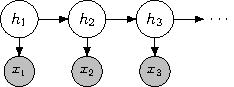
\includegraphics[width=0.45\columnwidth]{figures/hmm.pdf}
    \label{fig:examples-hmm}
  }
%  \subfigure[Directed grid model] {
%    \label{fig:examples-grid}
%    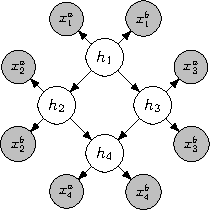
\includegraphics{figures/grid.pdf}
%  }
  \subfigure[Tree model] {
    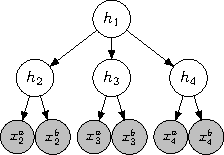
\includegraphics[width=0.45\columnwidth]{figures/tree.pdf}
    \label{fig:examples-tree}
  }
  \subfigure[Noisy-or model] {
    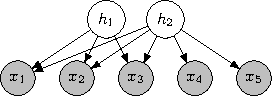
\includegraphics[height=5em]{figures/non-example.pdf}
    \label{fig:examples-noisy-or}
  }
  \caption{(a) and (b): graphical models that satisfy the exclusive views property;
  (c) a graphical model that does not.}
  \label{fig:examples}
\end{figure}


\paragraph{Example: hidden Markov model.}

In the HMM (\figureref{examples-hmm}),
$h_2$ is a bottleneck, so we can recover $O \eqdef \Pr(x_2 \mid h_2)$.
%the parameters
%are $O \eqdef \Pr(x_i|h_i)$ and $T \eqdef \Pr(h_{i+1} | h_i)$
%for all $i$.
While the first hidden variable $h_1$
is not a bottleneck,
it still has an exclusive view $x_1$ with respect to the clique $\{h_1,h_2\}$,
assuming parameter sharing across emissions ($\Pr(x_1 \mid h_1) = O$).

\paragraph{Example: latent tree model.}

In the latent tree model (\figureref{examples-tree}),
%the parameters
%are $\pi \eqdef \Pr(h_i)$, $T \eqdef \Pr(h_i | h_1)$ for $i \in \{2,3,4\}$,
%and $O \eqdef \Pr(x^a_i | h_i) = \Pr(x^b_i | h_i)$ for $i \in \{2,3,4\}$.
$h_1$ is not directly connected to an observed variable,
but it is still a bottleneck, with views $x^a_2, x^a_3, x^a_4$, for example.
The clique $\{h_1,h_2\}$ has exclusive views $\{x_2^a,x_3^a\}$.
%We can recover $T$ from the clique $\{h_1, h_2\}$ by using views $x^a_2$
  %(exclusive to $h_2$) and $x^a_3$ (exclusive to $h_1$).

\paragraph{Non-example}
\label{sec:non-example}

%There are certainly models which are identifiable but do not have exclusive views.
In \figureref{examples-noisy-or},
  $h_1$ does not have exclusive views.
  Without parameter sharing, the techniques in this paper
  are insufficient.
In the special case where the graphical model represents a binary-valued noisy-or network,
  we can use the algorithm of \citet{halpern2013unsupervised},
  which first learns $h_2$ and subtracts off its influence,
  thereby making $h_1$ a bottleneck.
